\section{System Implementation}
This section presents how the system was implemented. The system’s main parts are presented, after which individual parts will be explained in greater detail. This section also covers how the team implemented persistence, concurrency and role-based access control. \newline
The system was written and tested using the programming language C\# on the .NET platform
\subsection{Overview}
The following has been implemented in the final system:
\begin{itemize}
\item A peer-to-peer architecture which can be distributed across an arbitrary number of web services.
\item The workflow system is generic in the sense that it supports not only a single, built in workflow. Furthermore a workflow is able to dynamically change while it is running.
\item Workflow events have \textit{location transparency}; events can be held at different servers or at the same server. The internal logic does not differ across locations. 
\item A \textit{graphical user interface} that provides a more appealing user experience for the end user to interact with. 
\item \textit{History}, enabling the user to see a log of what happened at both the Server and at a single event.
\item \textit{Persistence}, if the machines running the Server or an EventAPI are shut down, once restarted they will be able to restore from where they left off.
\item Role-based access control, which ensures that a user is only able to execute events that the given user has permission to.
\item \textit{Locking} prevents simultaneous access to events. Simultaneous access could otherwise cause a corrupted state in a workflow. 
\end{itemize}
\subsection{Overall Architecture}
This section aims at providing a panoramic view of the architecture of the delivered system. \newline
Now, a brief explanation of the three main parts, that constitute the delivered software:
\subsubsection{Client}
The client is the software an end user will typically interact with when using the system. The Client was described in the Section  \ref{sec:Usermanual} \nameref{sec:Usermanual}. The user uses the Client to execute events in a workflow, reset a workflow, or see a history of what happened at the events and at the Server. The Client interacts with the Server and possibly several EventAPIs.
\subsubsection{Server}
The Server is a centralized instance that holds information about all workflows. For each workflow it provides the addresses of all events in the given workflow. The Server is contacted by the Client, when the Client wants to know what workflows exist at the Server and know what events are related to a specific workflow. \newline
Furthermore, the EventAPI also interacts with the Server, when an event wants to add itself to an already existing workflow at the Server. The Server is intended to be a REST-based service, see Section  \ref{sec:REST} \nameref{sec:REST} \newline
In the current setup, the Client has no way of discovering the Server automatically, and hence the Client is hardcoded to the address of the Server, stored in a configuration file. It is possible to have multiple Servers, however a workflow must be located at a single Server. Furthermore a Client can only contact one server per instance.

\subsubsection{EventAPI}
The EventAPI holds events and is responsible for the execution of events. The Client will contact the EventAPI when asking for the state of events. The EventAPI contacts the Server when events are created or deleted. EventAPI is a REST-service. \\

The three main subsystems and their interactions are sketched in the Figure \ref{fig:ThreeMainSubsystemsSketch}. 

\begin{figure}[h!]
\centering

\includegraphics[width=0.4\linewidth]{Figures/strawberry}
\caption{\label{fig:ThreeMainSubsystemsSketch} Illustration of the system's three main components and their interaction.}

\end{figure}
\subsection{Interface-based Programming}
\subsection{Dependency Injection}
\subsection{Design of Client}

\subsubsection{MVVM-principles in Client}
\subsection{Design of Server and EventAPI}

\subsubsection{Multi-layered Design}

\subsubsection{Execution of an Event}
\subsection{Distribution}
One of the requirements to the system was that it had to be distributed.
 
The intention was that events should be distributed across several EventAPIs. The fact that the Server is centralized could potentially create a performance bottleneck and the Server has therefore been developed to have as little responsibility as possible to minimize this issue. Reducing this bottleneck comes down to two things: Handling as few requests as possible and not doing heavy processing. The sooner a Client can be routed away from the Server to EventAPIs, the better. The Server supplies the Client with a list of events. From then on, the Client now communicates directly with EventAPIs bypassing the Server as a middle man.\\

Since events can be deployed on an infinite number of EventAPI instances, the system is distributed. Processing requests across several EventAPI instances - instead of just a single EventAPI - helps balancing the workload to avoid performance bottlenecks. 
Making the system distributed presented some problems which are explained in Section \ref{ConcurrencyControl} \nameref{ConcurrencyControl}

\subsubsection{Location Transparency}
The EventAPI has been designed in such a way that it does not distinguish between events located at the same EventAPI and events located at other EventAPI instances. The same logic is used for either case. \\

This implies that an EventAPI will issue a HTTP request to itself, even though the target event is located at the same EventAPI instance. 

Therefore, the team believes events have location transparency.

\subsubsection{\label{sec:GlobalID}Global Identification of Events}
An event is uniquely determined by the combination of its own ID (eventId) and the ID of the workflow the event belongs to (workflowId). Two events on the same workflow cannot share the same eventId. Therefore two events cannot share the same global ID. 
This property allows for an event to be uniquely determined in the system and it allows exposing a directory-like structure in the URLs as prescribed by REST - see Section \ref{sec:REST} \nameref{sec:REST}. 
EventAPIs locate their resources as such: \\

\begin{center}
$<$baseurl$>$/events/$<$workflowId$>$/$<$eventId$>$
\end{center}

As an example, the event \textbf{Read Gasmeter} belonging to the workflow Pay Gas would be located on the following URL:  

\begin{center}
\url{http://www.myRestService.com/events/PayGas/ReadGasmeter}
\end{center}


\subsubsection{System Deployment \label{sec:SystemDeployment}}
The nature of a distributed system means that it is running across several computers. Hosting the system on a cloud platform like Amazon EC2 or Microsoft Azure was an obvious choice. With the team’s chosen system architecture, the system requires the Server to be present. Hosting the Server in a fixed, known location makes communication between the Client, the EventAPI, and the Server easier. 

Choosing Microsoft Azure for hosting the system instead of other hosting platforms was simply a result of the convenience of using Azure. The platform has Visual Studio integration and Microsoft supplies students at the IT University of Copenhagen with a free hosting service that offers enough scalability for this project. The entire backend of the system is therefore hosted on Azure across several virtual machines. One virtual machine hosts the Server that Clients access when they first enter the system. Several EventAPIs are hosted across other virtual machines. 


\subsection{RESTful APIs}
This section covers to what extent the team believes the Server and the EventAPI are RESTful. API is here used to refer to the Server and the EventAPI. 

\subsubsection{Restfulness of the System}
The APIs exposes their resources through a RESTful interface. Creating objects in the system is done through HTTP POST requests. Updating objects and information is done using PUT requests. Retrieving information is done through GET requests, where the request has no information apart from URL request parameters.
 
No knowledge of the implementation of the APIs is accessible from outside the system. Only incoming and outgoing information is accessible unless stated below. 

Users of the APIs do not need to know about the internal state and representation of data in the APIs. Users of the APIs send and receive information in Data Transfer Objects - DTOs - as JSON.\\

The APIs act as resource providers that provide information when requested to do so, without needing to know anything about the users of the APIs and vice versa. 

RESTful layering is also present in the implementation in the sense that a user of the APIs at no given time knows whether it is communicating directly with an API or whether the request is handed to an intermediary.

\subsubsection{UnRESTful Parts of the System}
Some behaviour at the APIs cannot be described as RESTful. The \texttt{Execute} method on the EventAPI's \texttt{StateController} is one example. The intent of this method is to execute an event. 

\texttt{Execute} is called with a PUT request. A PUT request should replace the targeted resource with the resource provided in the request. However, \texttt{Execute} does not. The resource that is given in the PUT request is instead used as input for executing the method. 

The central problem is that the execution of an event hardly corresponds to a resource, instead it is an operation that the caller wants the EventAPI to carry out. 

The second problem is that this deviation propagates to the caller of the EventAPI as well. 
Now the caller also needs to know that the method should be invoked through a non-compliant HTTP PUT request. Now there is coupling between the implementation on EventAPI and how clients should invoke \texttt{Execute}. Architecturally this resembles SOAP\footnote{\url{http://en.wikipedia.org/wiki/SOAP}} more than REST, since it is function based.\\

A possible fix for this would be to PUT some sort of Execute resource to a given event, which would then be stored on the event after execution. It could be argued that a resource is then simply stored at the event even though the state of the event changes.
\subsection{Minimal Logic Handling in Controllers}
The following section describes the implemented structure of the controllers in the Server and the EventAPI. Controllers across the EventAPI and the Server share architectural similarities since both are implemented as REST web services. \\

During the implementation of the Server and the EventAPI it was a design goal for the Controllers to do as little work as possible besides receiving the incoming HTTP requests and checking for invalid input. \\ 

It was therefore the intention of the design that controllers should only have the following four responsibilities:
\begin{itemize}
\item Checking that input can be converted into an instance of the given argument type
\item Delegate the call to a logic layer
\item Catch and form relevant exceptions which is mapped to HTTP responses
\item Request a history entry to be recorded in all three cases
\end{itemize}

As far as possible the controllers should not handle any logic, but instead simply pass on the incoming information to another layer that will then process and return the necessary information. This ensures encapsulation of responsibility and enables the use of several smaller classes for handling domain-specific logic. The team aimed for several controllers, since one big controller with a lot of different functionality is hard to test and reuse.\\

An implementation of the aforementioned design intention is presented below, see Figure \ref{fig:LockController}.

\begin{figure}[h!]
\centering
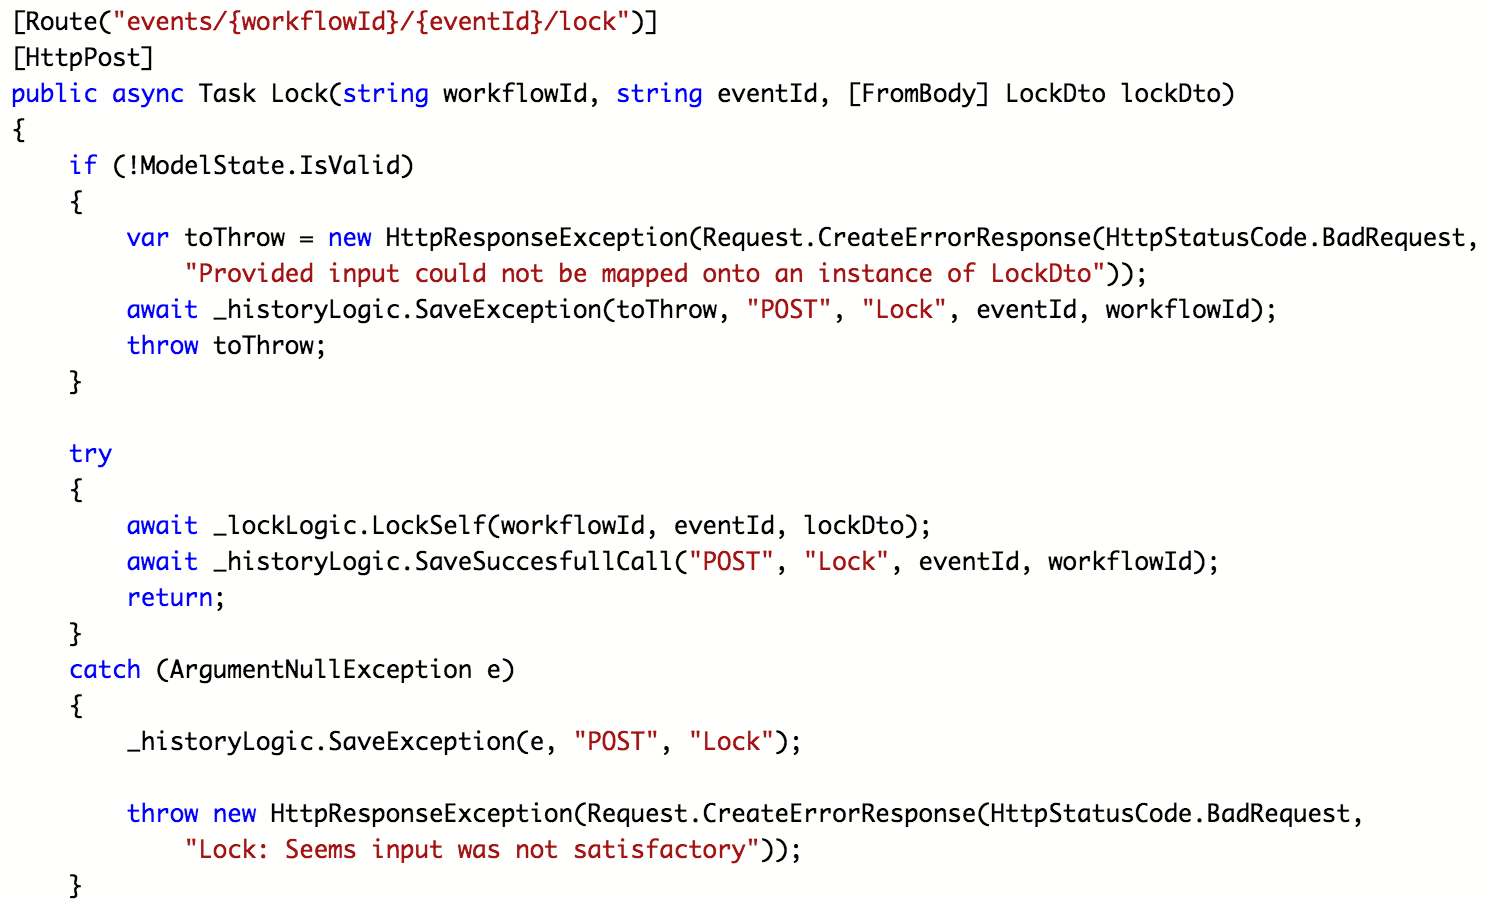
\includegraphics[width=\linewidth]{figures/LockController}
\caption{\label{fig:LockController}A code snippet from \texttt{LockController} in EventAPI. \texttt{Lock} checks for input validity, and if it is valid, it delegates the work to the \texttt{LockingLogic} layer. The try-catch design will be discussed in the following section. }
\end{figure}


\subsubsection{Exception and Response Handling}
First of all, there are a number of exceptions that may arise through the execution of an HTTP request. The team's exception handling approach comes down to distinguishing between two types of exceptions. Those that can be handled locally and those where the exception are propagated all the way up to the controller level. In a given scenario the responsibilities of the involved components determine the scenario type. 

In the following subsections the handling of either of these two types of exceptions will be elaborated.

\paragraph{Exception is Handled Immediately}
If an exception can be dealt with locally and the upper layers do not need to know about what caused the exception, an action is taken accordingly. An example of such an exception scenario is found in the logic layer. Assuming an event during execution has locked four out of six related events, but when attempting to lock the fifth an exception is thrown. The logic must unlock the four locked events before returning to the caller. In this scenario the logic layer can - and should - deal with the exception. The requested operation cannot be completed and therefore a “clean up” by unlocking the four events.\\

The implementation of this is presented below, see Figure \ref{fig:LockList}.
\begin{figure}[h!]
\centering
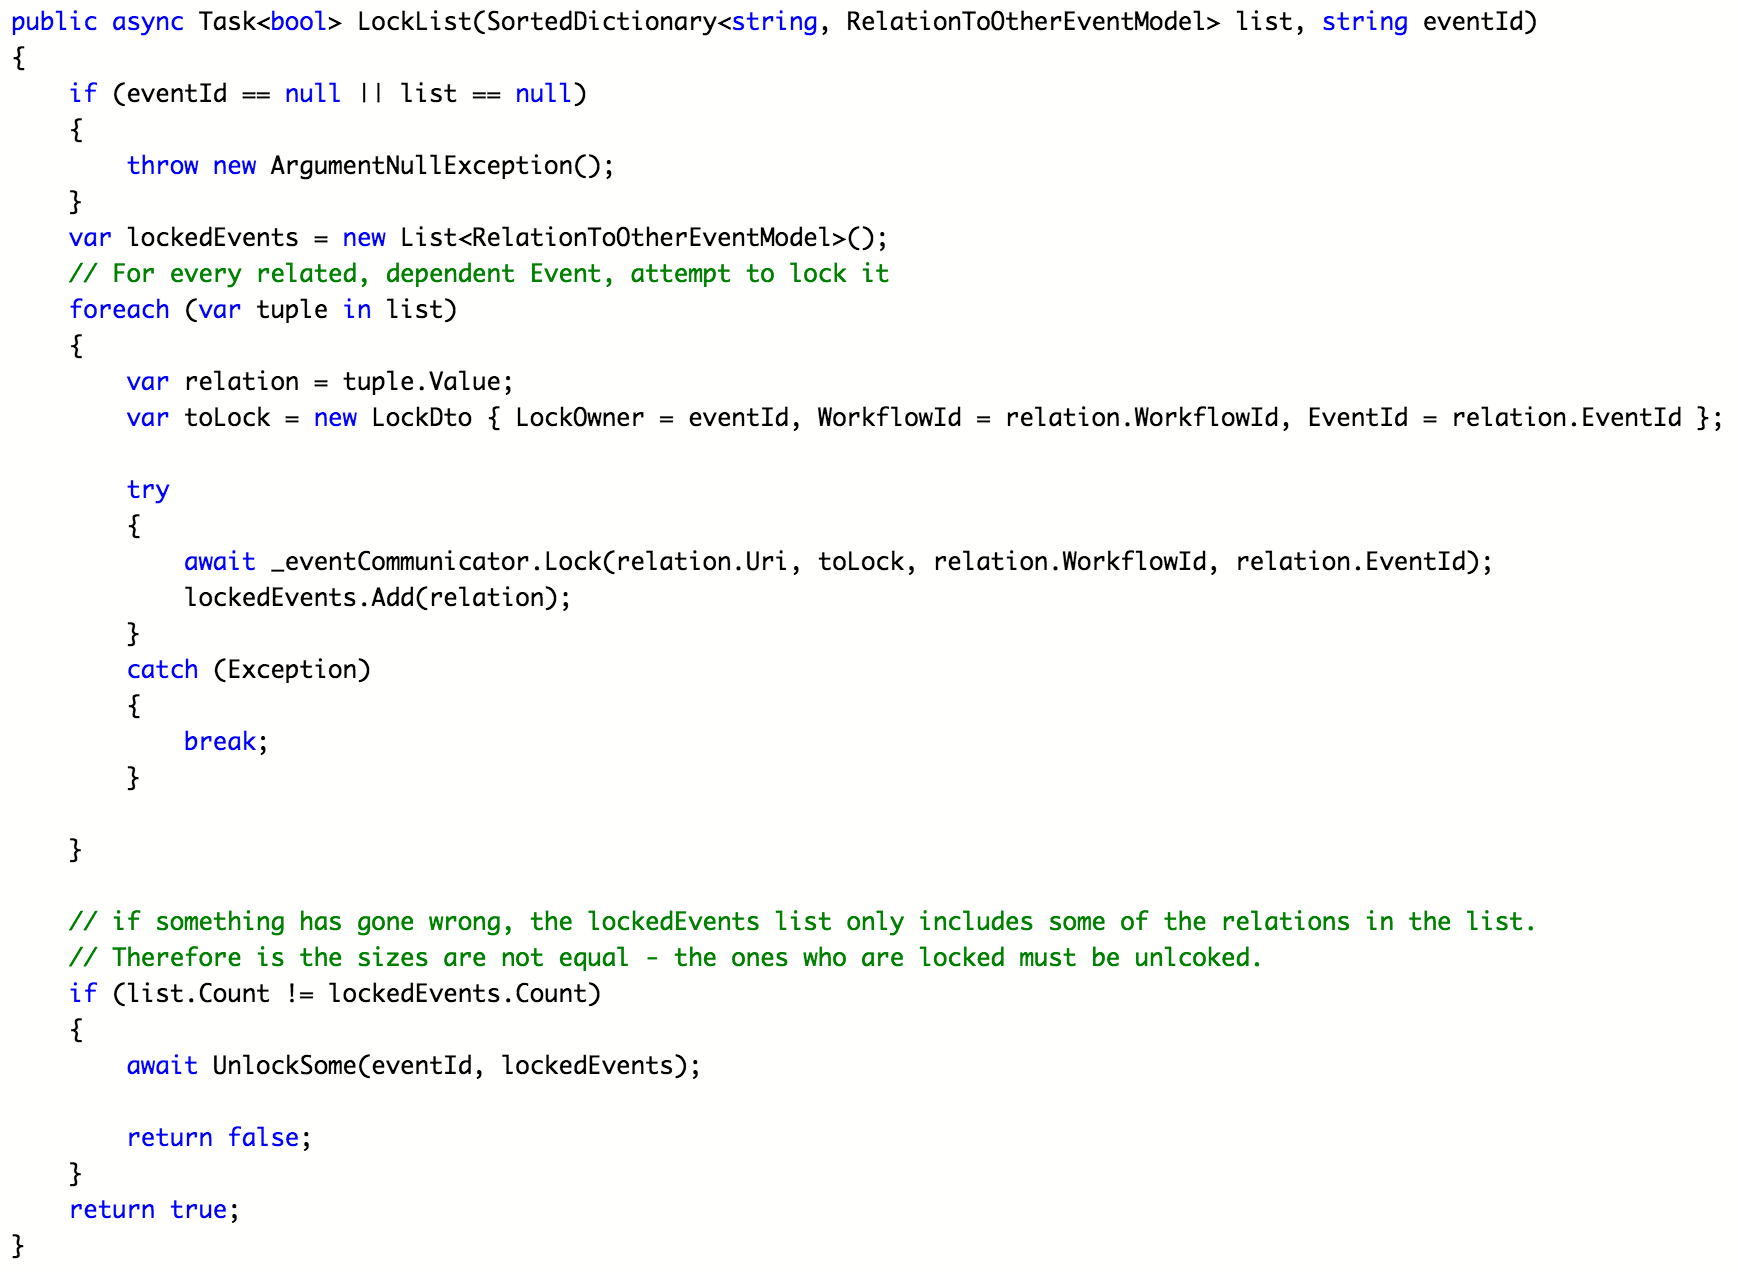
\includegraphics[width=\linewidth]{figures/LockingLogic}
\caption{\label{fig:LockList}Code-snippet from \texttt{LockingLogic} \texttt{LockList} method. Example of an exception that are thrown in modules below the LockingLogic layer, but are handled locally. Local exception handling is performed because the layer can actually do something about the exception. }
\end{figure}

\paragraph{Exception is Propagated Upwards}
If it is not possible for a layer to take proper action when an exception is thrown, it is propagated upwards to a layer which has interest in and can handle the exception.
When an exception occurs and the operation has to abort, the user of the Server or EventAPI must be notified of the error. 

In these scenarios there really is no obvious action to take in the lower layers. In some cases it is even possible for a layer to wrap the existing exception in another exception type which provides more information to the calling layer. If an exception is propagated to the controller layer, an appropriate HTTP response, based on the exception, is sent to the caller.\\

For instance, if a request is made to create an event with an ID identical to the ID of an already existing event, no countermeasure besides returning a bad request response to the caller exists. The lower layer should not determine what to do here, and therefore it propagates the exception upwards to the upper layer. \texttt{HttpResponseExceptions} thrown by the controller layer results in an HTTP error code being returned to the caller to give an idea of what went wrong.

\begin{figure}[h!]
\centering
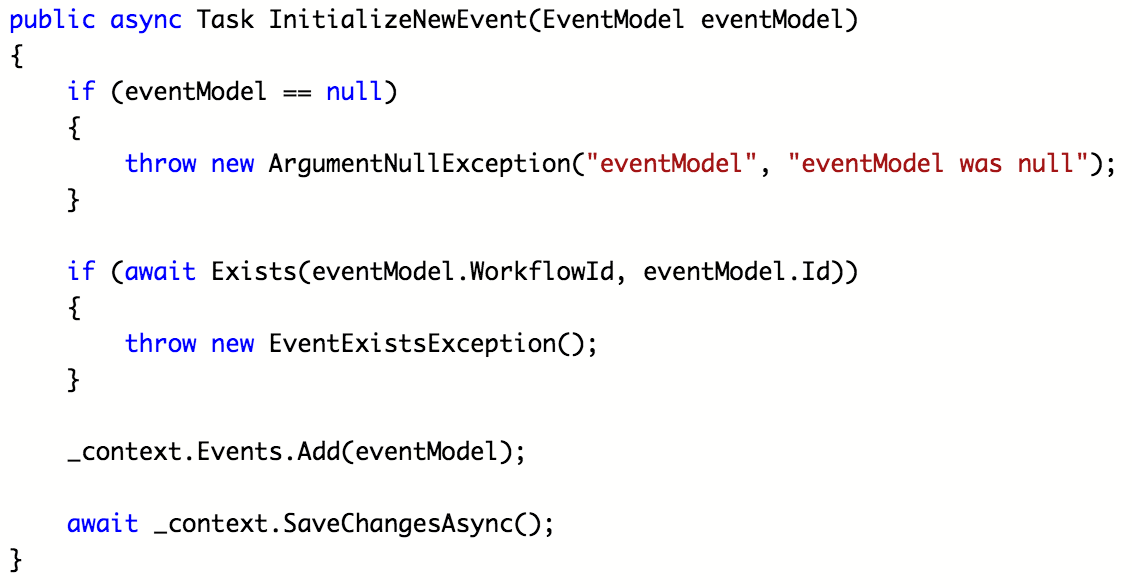
\includegraphics[width=\linewidth]{figures/EventStorage2}
\caption{\label{fig:InitializeNewEvent}Code-snippet from the method \texttt{InitializeNewEvent} in \texttt{EventStorage}}
\end{figure}

In the code-snippet seen in Figure \ref{fig:InitializeNewEvent}, it is realized that the event that is to be created have already been created. An \texttt{EventExistsException} is therefore thrown. This exception is then allowed to propagate up to \texttt{LifecycleController}, seen in Figure \ref{fig:CreateEvent}, where it is caught. The catching of the exception ultimately leads to \texttt{LifecycleController} issuing a bad request response. 

This also explains the need for the try-catch blocks pointed out in the previous section.  Note that catching different exceptions lead to slightly different HTTP response exceptions being issued to the caller each with a more descriptive error message than a default error message.

\begin{figure}[h!]
\centering
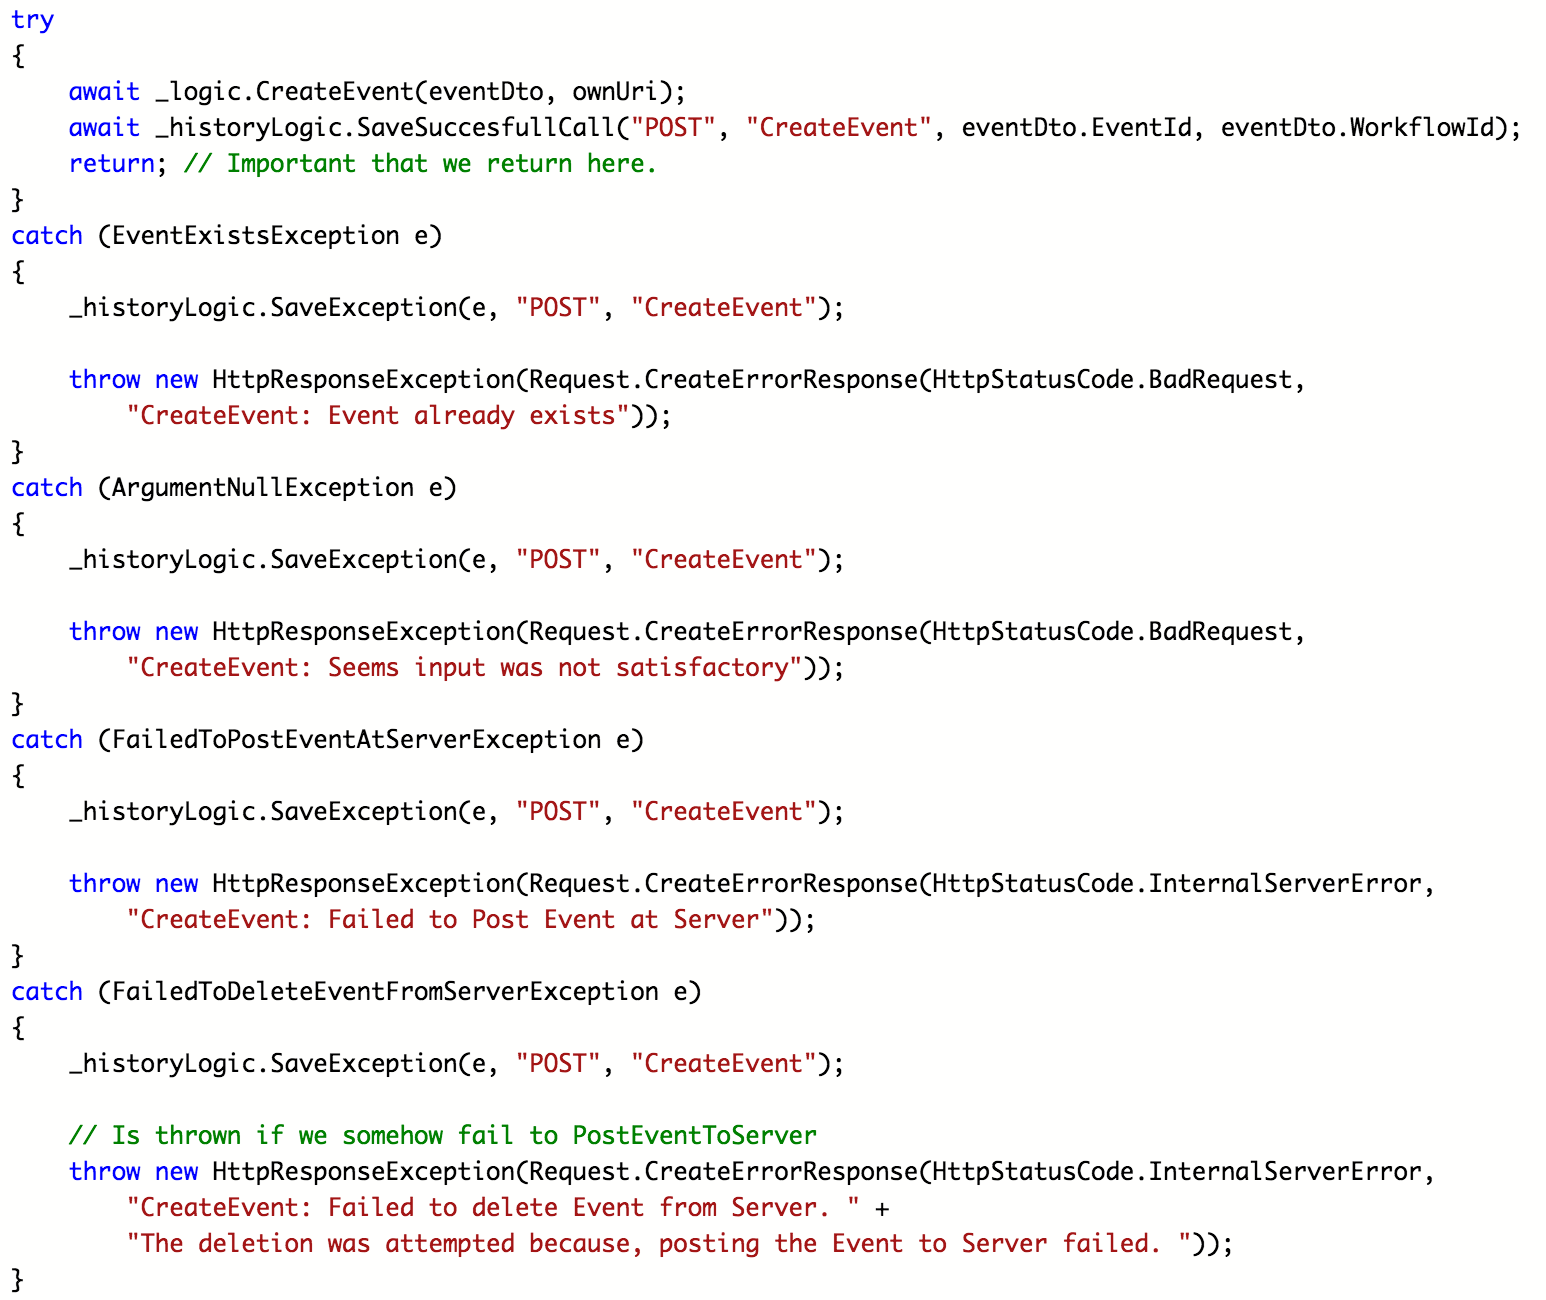
\includegraphics[width=\linewidth]{figures/LifecycleController}
\caption{\label{fig:CreateEvent}Code-snippet from the method \texttt{CreateEvent} in \texttt{LifecycleController}}
\end{figure}

It is important to note that with this approach the decision on what type of response to issue back to caller is made at the controller layer. \\

One could imagine an alternative approach where the throwing layer - in this case \texttt{EventStorage} - would decide on what response to return. This would break the encapsulation of the class since a lower layer would interfere with the responsibilities of a higher layer. 

By throwing an exception stating what the issue was at the lower level and then let top layers handle the exception, we encapsulate the responsibilities of the layers.
\subsection{Persistence}
This section describes how the finished system achieves persistence on the Server and the EventAPI. In this section an entity refers to the in-memory representation of a row in a relational database.\\

Data persistence is needed in case of system crashes or restarts. Therefore both the Server and the EventAPI implement data persistency in the form of an SQL database. 

To map a relational data model to in-memory objects Microsoft's Entity Framework was used. By having persistent data, the system became more robust. This became more apparent when the deployment on Microsoft’s Azure hosting platform was taken into consideration. Azure will shut down the deployed Server and EventAPIs when not in use. Resuming from a stored state is therefore a necessity if data should not be lost.  

\subsubsection{The Relational Database}
To persist data of events and workflows on both the Server and the EventAPI two relational data models were created. When mapping objects to relational data the concepts of redundancy and normalization were used.

Data models are only used in the storage layer of the subsystems. POST and PUT requests with DTOs are converted to entities by a logic layer and are finally persisted. 

Similarly GET requests requires the logic to retrieve entities from the database and convert them to the wanted DTOs which can then be sent with a HTTP response. 
Data independence was achieved by having different kinds of data - data for transferring,  DTOs, and data for saving, entities. This enabled implementing new DTOs or easily adding data to an existing entity without changing anything in the DTOs.\\

The data model of the EventAPI contains seven models, and can be seen on Figure \ref{fig:EventAPIDataModel}. The History entity has no relations to other entities which is intentional, because History data should not be deleted - even if an event is deleted. Furthermore, four models are created - one for each type of graph relation. This design choice was made to be able to extend the relations individually in the future. These models derive from the same base class and it is therefore easy to extend all of them simultaneously. 

The three fields \textit{InitialExecuted}, \textit{InitialPending}, and \textit{InitialIncluded} on the Event model are used to reset an event to its initial state. Multiple roles on an Event are allowed which is seen on the one-to-many relation from Event to Role. 

Notice that an Event has a composite key of the WorkflowId and EventId - two events can have the same Id as long as they do not exist on the same workflow - see Section \ref{sec:GlobalID} \nameref{sec:GlobalID}.\\

\begin{figure}[h!]
\centering
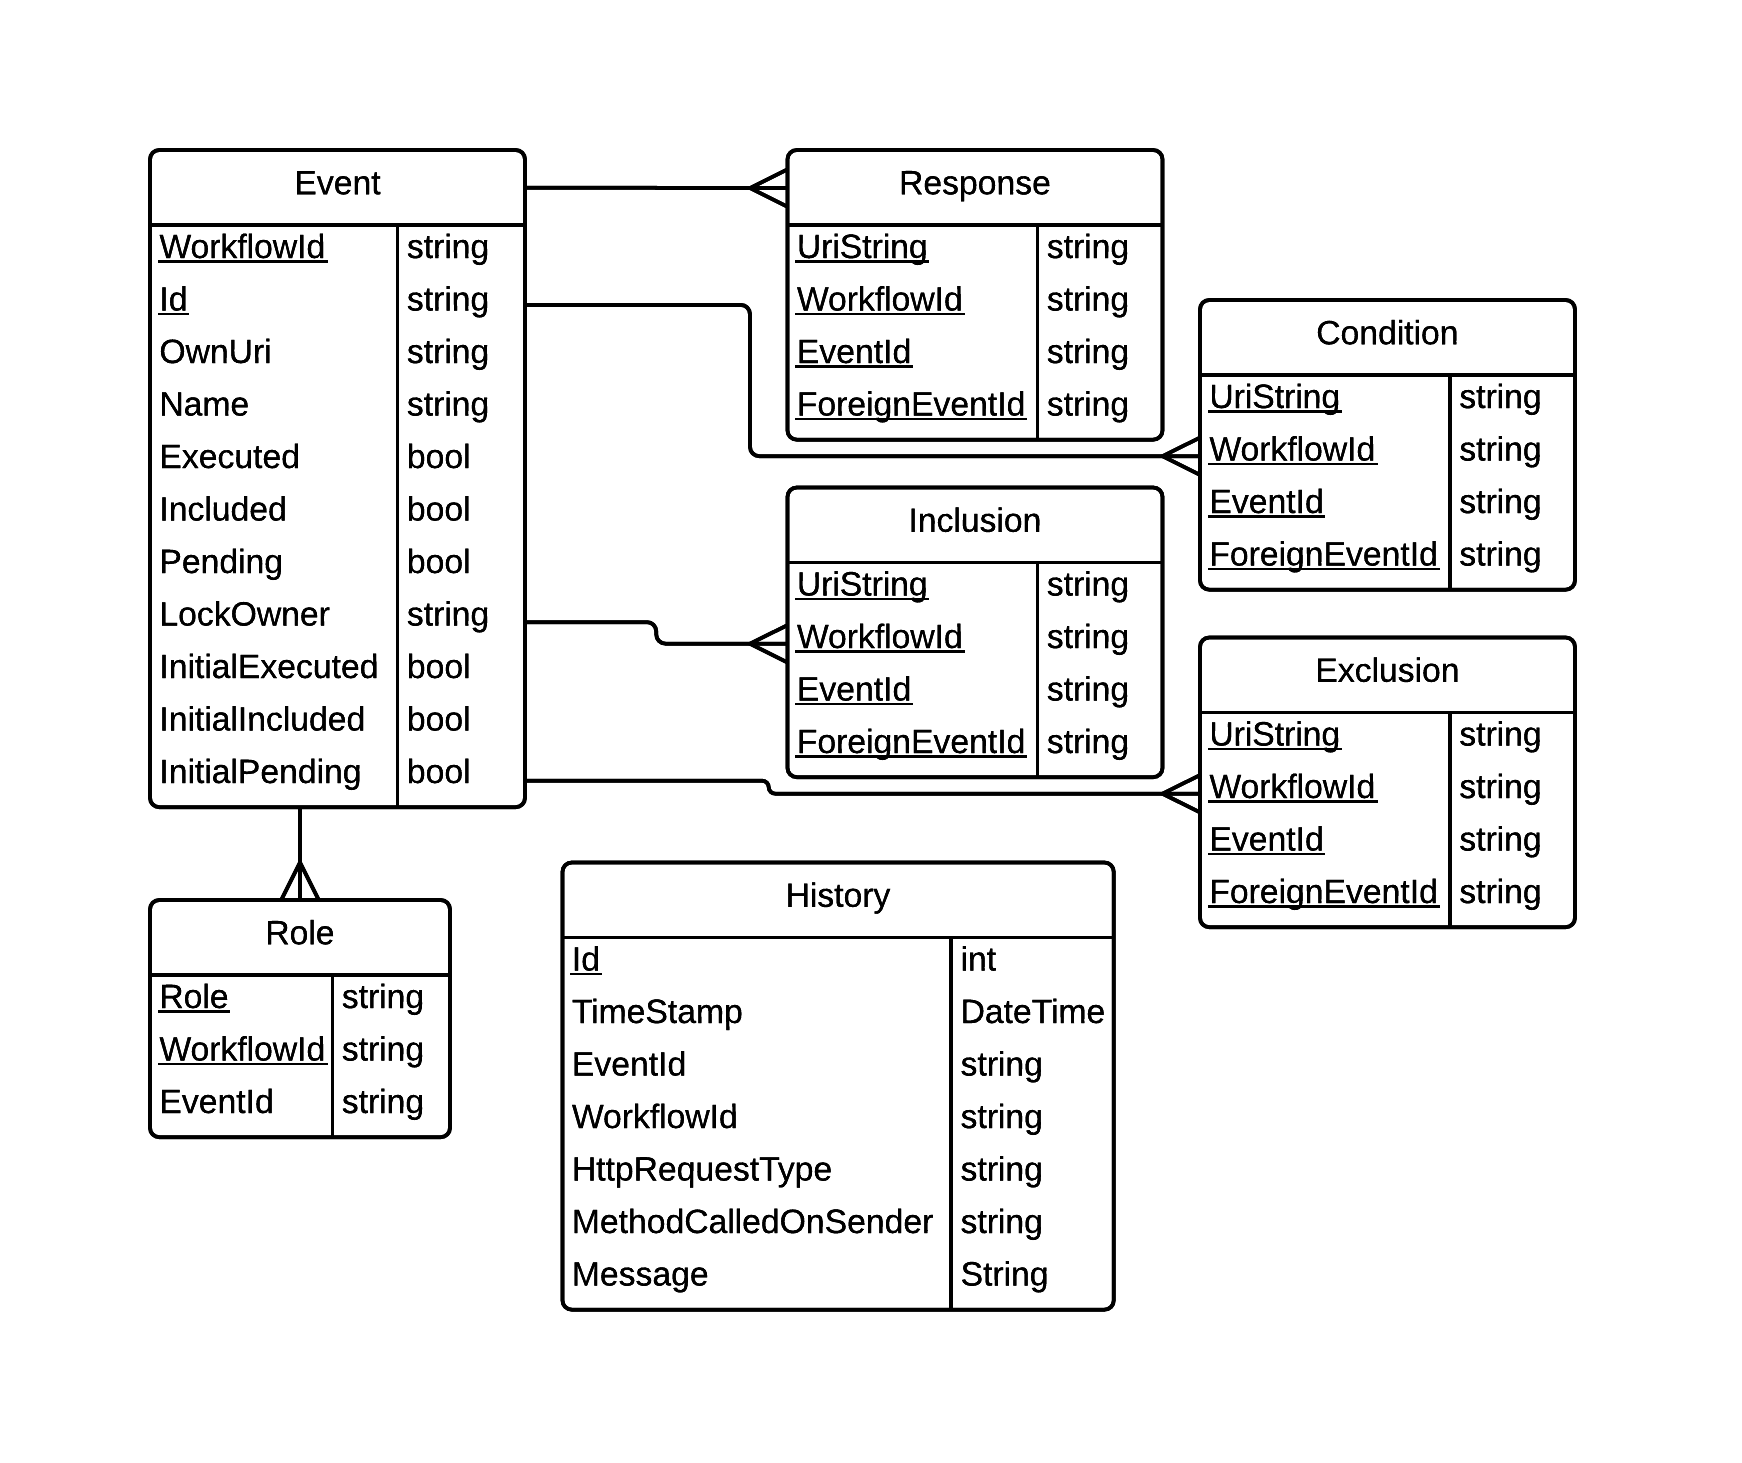
\includegraphics[width=\linewidth]{figures/DatamodelEvent}
\caption{\label{fig:EventAPIDataModel}The Data Model of an EventAPI}
\end{figure}

The data model of the Server can be seen in Figure \ref{fig:ServerDataModel}. The data model contains seven entities. 

\begin{figure}[h!]
\centering
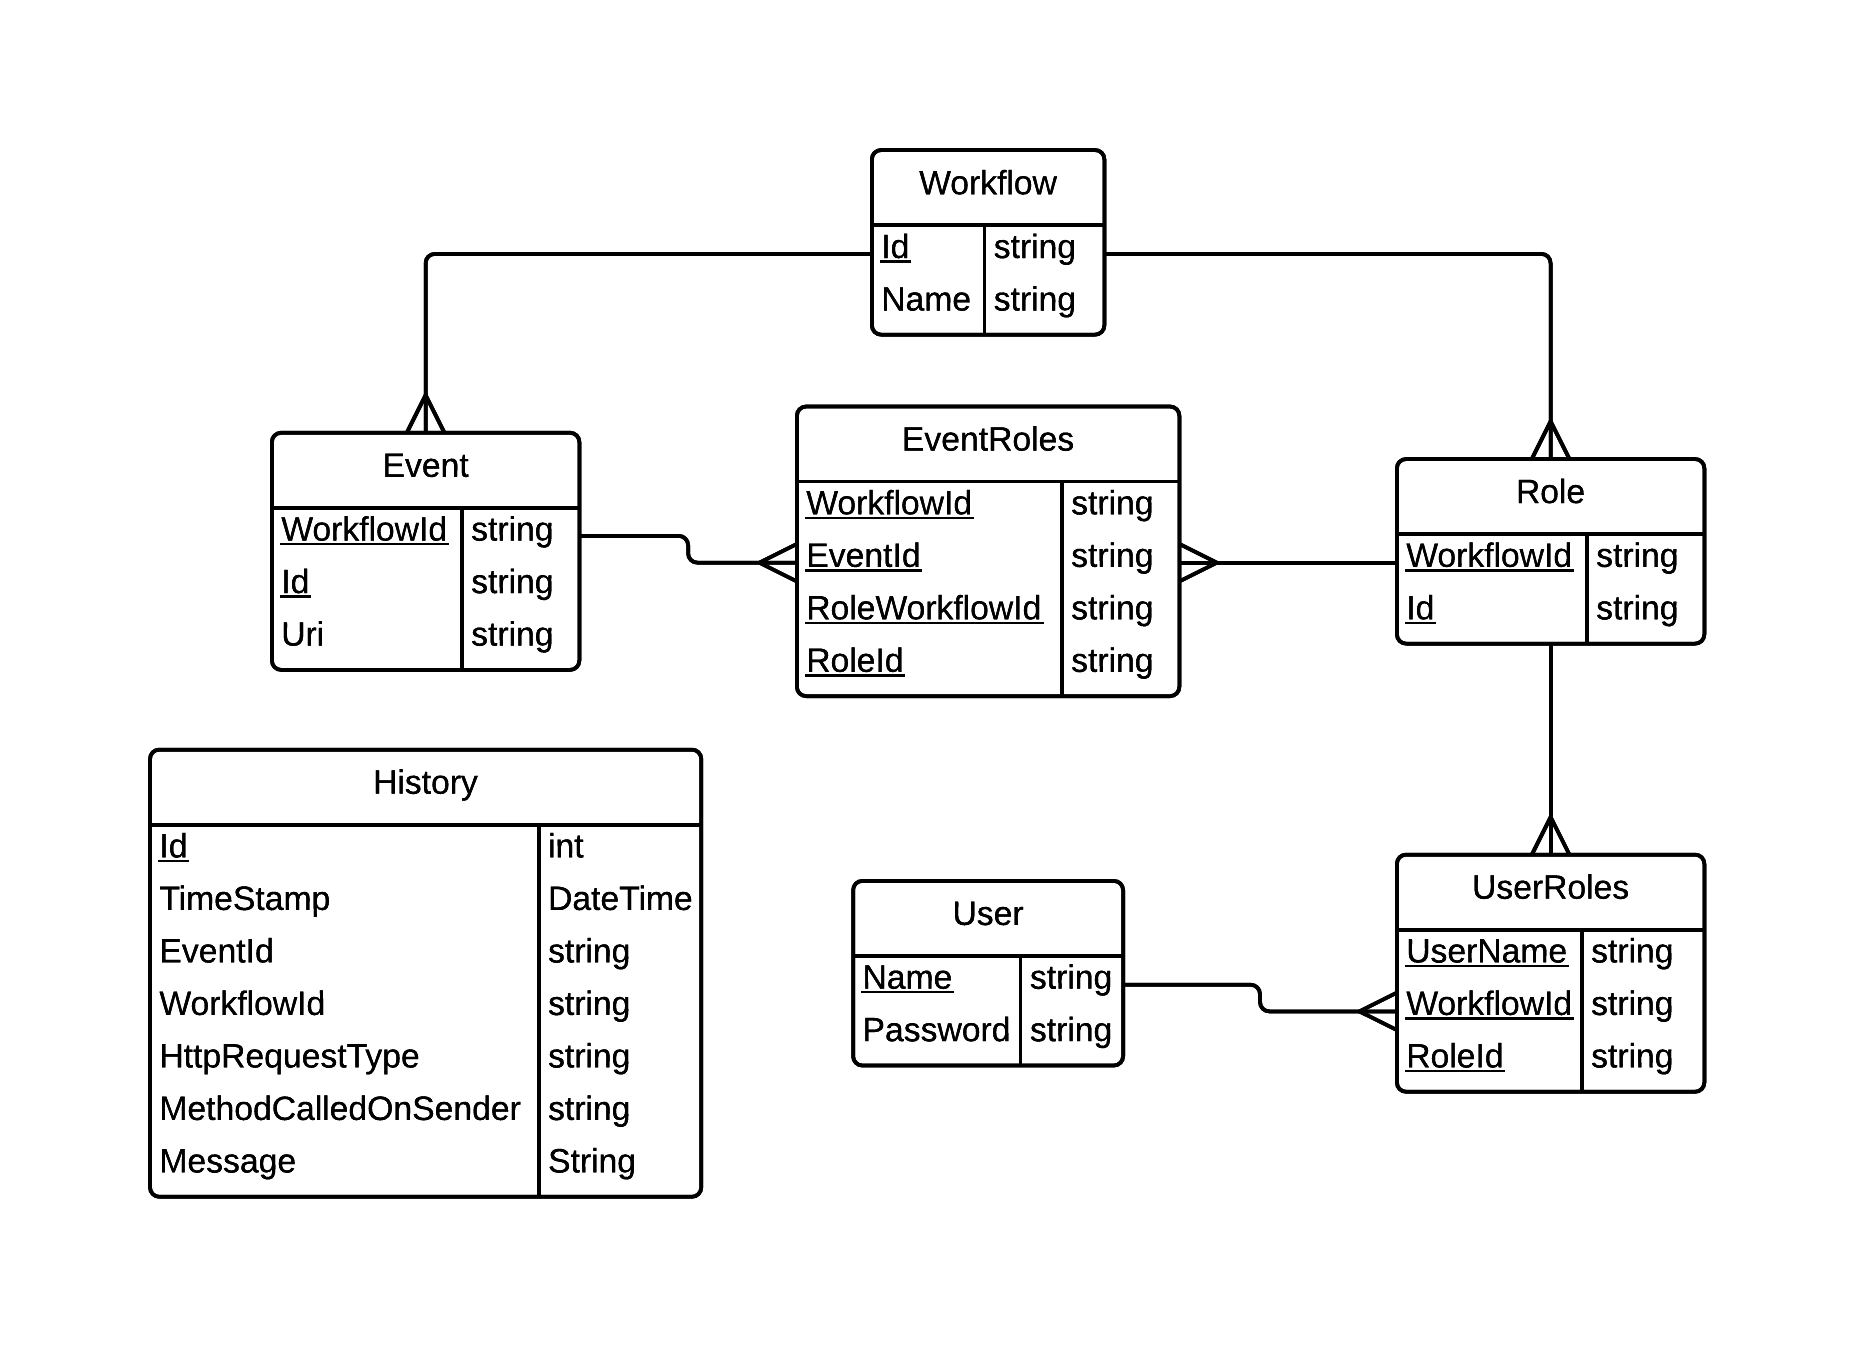
\includegraphics[width=\linewidth]{figures/EFDatamodelServer}
\caption{\label{fig:ServerDataModel}The Data Model of the Server}
\end{figure}

Notice the EventRoles table. This table is created to normalize the many-to-many relation between events and roles. The EventRoles entity is never used outside of the database. This entity helps Entity Framework minimize the amount of redundant data. The model allows for an event to have many roles and roles to be on many events, but a role is unique for a workflow. 

Since two events should be able to have the same ID on two different workflows, the Event model has a composite key of the WorkflowId and EventId. 
To support role-based access control a hashed and salted password for each user is stored, see Section \ref{sec:RBAC} \nameref{sec:RBAC}.

\subsubsection{Data Distribution}
The aforementioned data models allows storage of workflow and event information on the Server and the EventAPI, respectively. By storing data in multiple locations a bottleneck is removed since all data does not have to be stored and retrieved in one place. \\

On the Server, by only storing where to find events, but not any information about the state of each event, the Server and events are encapsulated since the Server has no need to know the state of individual events. An event keeps track of its own state, the Server simply serves event addresses. 

Furthermore, fewer errors are encountered by not saving copies of states of related events on each event. Instead events are forced to request data each time they need it. This, once again, encapsulates events and their responsibilities. It should be noted that this benefit comes at the cost of a performance impact.\\

By distributing data it is not possible to get access to all of the data of events at once and get an overview of the stored information of every event. This can function as a defense mechanism if an attacker would want to access all the data in the system. 
A problem with distributed data is that the roles of the system - when using role-based access control - have to be agreed on systemwide, which complicates matters. 
\subsection{\label{sec:RBAC}Role-Based Access Control}
This section describes how RBAC was implemented in the delivered system. RBAC is implemented across the system. Server, Client, and EventAPI all handle roles and in conjunction make RBAC possible.

\subsubsection{Motivation}
Without RBAC any user would be allowed to execute any event within a workflow. This would allow for troublesome and unintended effects. Examples of this could be drug addicts prescribing themselves morphine or taxpayers approving their own annual statement. 

RBAC will prevent users who cannot prove that they have one of the roles required from executing the event. For instance, in the workflow "Pay Annual Gas Bill", only users who can prove themselves to be a \textit{Customer} would be allowed to execute the \textbf{Read Gas Meter} event.

In short, because events within a workflow are assigned only to some roles, the system needs a way of ensuring that only people assigned with these roles are allowed to execute the given events. This was the motivation for implementing role-based access control. 

\subsubsection{Implemented Solution}
In the finished system a user can be assigned multiple roles and an event supports execution by multiple roles. This was implemented to make it easy to parse exported graphs from \url{DCRGraphs.net} into system events. \\

In the relational database of the Server, user passwords are hashed with the SHA-512 algorithm to ensure that no sensitive information is stored in clear text. 

Furthermore, to secure against dictionary attacks \footnote{\url{http://en.wikipedia.org/wiki/Dictionary_attack}} the passwords are salted by adding a few randomly generated characters in front of all the passwords before and after they are hashed.\\

The way the system implements role-based access control is such that a user issues a login call to the Server with a username and password. The Server will then retrieve the user by username, hash the provided password, and try to match the provided hashed password against a salted hash retrieved in the database of the Server. 

If a match is found the server will send a list of the roles assigned to the user to the Client. Roles are defined in the workflow a given event belongs to, which means that multiple workflows can share role IDs without giving unwanted access to the wrong users.\\

The Client receives a dictionary of roles, where the key is the ID of the workflow and the value is a list of roles for the given workflow.

When the Client retrieves the addresses of events from the Server, the Client is able to discard the events on which the user has no execution rights, due to the fact that the Server will map an event to the roles the event supports.\\

During implementation it was also determined that users should not be able to be given roles that are not used by events in a given workflow. 

This limits the possibility of users getting access to events not assigned to them because an administrator of the given workflow did not check the current database for unused roles. Roles are not removed from the server when it is no longer in use. In this scenario it is possible for a user to be assigned an unused role.

\subsubsection{Discussion of the Implemented Solution}
The implemented solution is not ideally secure. All communications are sent via the HTTP protocol which transfers data in clear text. HTTPS could have been enforced but was not done due to HTTPS warnings caused by using self signed, and therefore untrusted, certificates. \\

Roles are also sent as JSON, which means that everyone with some insight into the implementation of the system could forge a list of roles and try to execute an event using that list, or simply just copy the roles from an intercepted request. One way to overcome the latter problem is to encrypt the list of roles, and send the encrypted access rights instead. This solution requires a shared secret which is only known to the Server and the EventAPI. The use of asymmetric encryption could also be used such that the access rights would include a value which would uniquely identify the Server. This value would then be encrypted so that only EventAPIs could read it and verify that the access rights were from the Server. The latter solution can pose problems because the server should deliver a unique value for every EventAPI, as they should not share encryption keys. The lifetimes of these access rights and unique values should also be limited because the longer a secret is used the greater the risk of its misuse will be.\\

"Distributed Systems - Concepts and Design"\footnote{Distrubuted Systems - Concepts and Design p. 475} mentions a way to login where the password is never transmitted over the network. This method makes the client send a request containing a username to login at a server. The server then responds with the access rights which are encrypted with a key that can be derived from the password.
\subsection{\label{ConcurrencyControl}Concurrency Control} 
This section will describe the motivation for having concurrency control, which solutions were considered, and the solution that was ultimately implemented.\\

Two major solutions to concurrency control are in use in software today: pessimistic concurrency control\footnote{Distributed Systems - Concepts and Design p. 692} (PCC) and optimistic concurrency control\footnote{Distributed Systems - Concepts and Design p. 707} (OCC).\\

PCC uses the concept of locking which prevents multiple transactions from accessing shared data simultaneously. OCC on the other hand uses a working copy of shared data to carry out a transaction and the changes are validated before possibly committing. If a transaction discovers a conflict between itself and a concurrent transaction, the implementation will decide which transaction aborts.

\subsubsection{Motivation}
\subsubsection{Implemented Solution}
The chosen concurrency control method was PCC. The implementation uses strict two-phase locking. At first a growing phase is carried out, in which the event will try to lock every other event it needs to complete the transaction. The event will then execute, update the states of the relation, and finally release all locks. 

If the event fails to acquire the needed locks in the growing phase it will abort the transaction by unlocking events that were locked in the growing phase. 

Strict two-phase locking ensures that the order in which the transactions are completed will be serially equivalent as well as preventing certain situations where deadlocks could otherwise occur.

If an event is locked, both reads and writes are delayed until the event is unlocked. Reading of an event is not allowed before the event is unlocked, because of the assumption that if an event is locked then it will almost certainly change its state and therefore affect the read values.\\

To prevent transactions from aborting, e.g. if they have to acquire a lock on an event which has already been locked, a "First In First Out" queue of lock requests has been implemented. 
When an event is unlocked, the next request in the queue, if any, will lock the event if it requires to update the state of the event. Reads, as mentioned, do not lock the event. This is due to the fact that read operations do not conflict each other in PCC.

If it takes more than ten seconds to acquire read or write access, the request will abort and the system will return a timeout exception to the caller.\\

To prevent deadlocks a global order in which the events will acquire locks have been implemented. The order is alphabetical and is based on the \textit{eventId}. As the event itself is in the ordered list, it is locked in the global order as well. The order of unlocking is not important as long as the executing event unlocks itself last. If an event unlocked itself before others, it might be prevented from unlocking the other events. \\

With this approach deadlocks will never be encountered as every event has to lock in the same order. Argumentation for why this works is given in the next section.
\subsubsection{Discussion of Implemented Solution}